\nuovapagina

\vs(5)
{\normalsize \bf Fase 2)}\\
\vs(3)
{\normalsize \bf Modello del contorno attivo - snake}

\fbox{
\noindent
\begin{minipage}{16cm}
\vs(2)
\center
{\normalsize Rappresentazione a B-splines cubiche uniformi della curva}\\
\vs(5)
\bfl
La curva \e ottenuta come composizione di segmenti di funzioni polinomiali o {\it spans}
descritti in generale dalla mappa
\vs(5)
\be
{\bf x}_i(u,t)\,=\,\sum_{j=0}^{N_B-1}\,B_i(u)\,{\bf q}_i(t)
\ee

\vs(10)
dove $B_i$ sono le {\it funzioni base} dello spazio 
e ${\bf q}_i$ i {\it control points}.

\vs(10)

\centerline{
 \psfig{file="./images/conv_h1.eps",height=8cm,clip=}
}
\vs(10)
\efl
\end{minipage}
}

%========================================================================================
\nuovapagina

\vs(5)
{\normalsize \bf Modello del contorno attivo - snake}

\fbox{
\noindent
\begin{minipage}{16cm}
\vs(2)
\center
{\normalsize Rappresentazione a B-splines cubiche uniformi della curva}\\
\vs(5)
\bfl

\vs(20)
Propriet\a:
\vs(10)
\bi
\im compattezza: la curva \e interamente definita dai suoi control points
 \vs(10)
\im controllabilit\a locale: variando la posizione di un control points si modifica solo una 
    parte della curva
 \vs(10)  
\im invarianza alle traslazione e in particolare alle omotetie (dilatazioni)
 \vs(10)
\im \e possibile esprimere le diverse misure in funzione dei soli control points
\ei
\vs(20)
\efl
\end{minipage}
}


%========================================================================================
\nuovapagina
\vs(5)

{\normalsize \bf Modello del contorno attivo - snake}

\fbox{
\noindent
\begin{minipage}{16cm}
\vs(2)
\center
{\normalsize La funzione energia e la legge di evoluzione dello snake}
\vs(10)
\bfl
Data la funzione vettoriale delle primitive $P$

\vs(10)
\centerline{
 \fbox{
 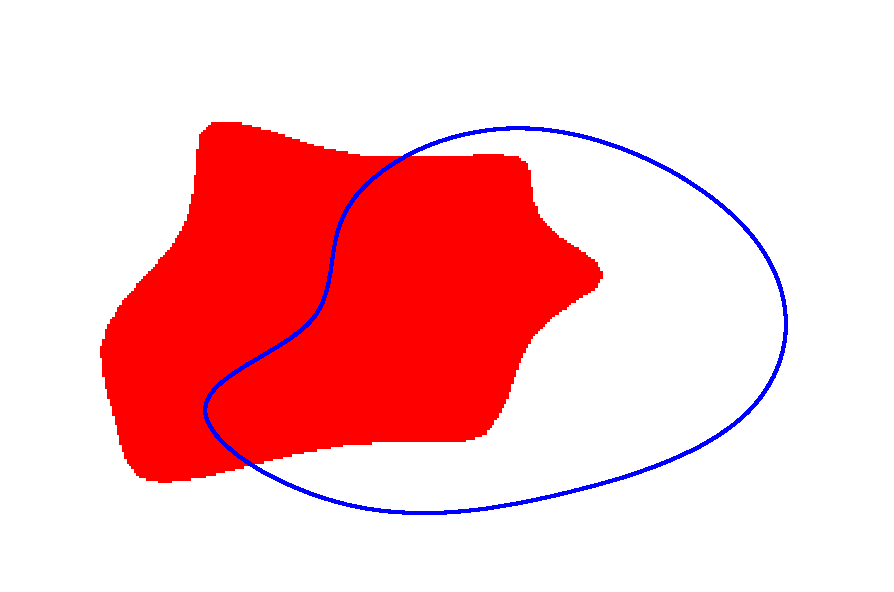
\psfig{file="./images/Eyezzi.eps",height=6cm,clip=}} 
}

\vs(10)
la funzione energia potenziale per immagini bimodali, rispetto a $P$, \e 
[{\it Yezzi et al. 1999}]:
\be
{\cal E}\,=\,-\,\frac{1}{2}\,\|m^{int}-m^{est}\|^2 
\ee
con $m^{int}$ e $m^{est}$ medie interne ed esterne rispetto alla curva.
\vs(3)
\bi
\im Permette di combinare caratteristiche dell'immagine diverse tra loro in modo semplice
    (ad esempio contemporaneamente colore e tessitura)
\ei
\vs(5)
\efl
\end{minipage}
}




